\graphicspath{{images/program}}

\section{Programm}

% In diesem Kapitel wird das Programm beschrieben, welches die Fotobox steuert.
% Zuerst grober aufbau mitteld diagramm und beschreibung einzelner komponenten.
% Dann in späteren kapiteln genauere beschreibung.

Das gesamte Fotoboxsystem besteht aus mehreren Komponenten, die möglichst nahtlos
miteinander Arbeiten, um dem Benutzer eine einfache und intuitive Bedienung
zu ermöglichen. 

Im Zentrum steht das Windows-Programm, das die Steuerung der Kamera und des
Druckers übernimmt. Es zeigt das Livebild der Kamera auf dem Laptop an,
verarbeitet die aufgenommenen Bilder und sendet sie an den Webserver.

Ein weiterer Bestandteil ist der Webserver. Dieser organisiert die
aufgenommenen Fotos, stellt eine Benutzeroberfläche bereit, über die die Fotobox
konfiguriert werden kann, und ermöglicht den Download der Bilder.

Das Zusammenspiel dieser Komponenten sowie deren genaue Funktionsweise werden
in den folgenden Kapiteln im Detail erläutert.

\newpage

\subsection{Desktop Applikation}

In dem folgenden Kapitel wird die Desktopapplikation 

\begin{figure}[H]
    \centering
    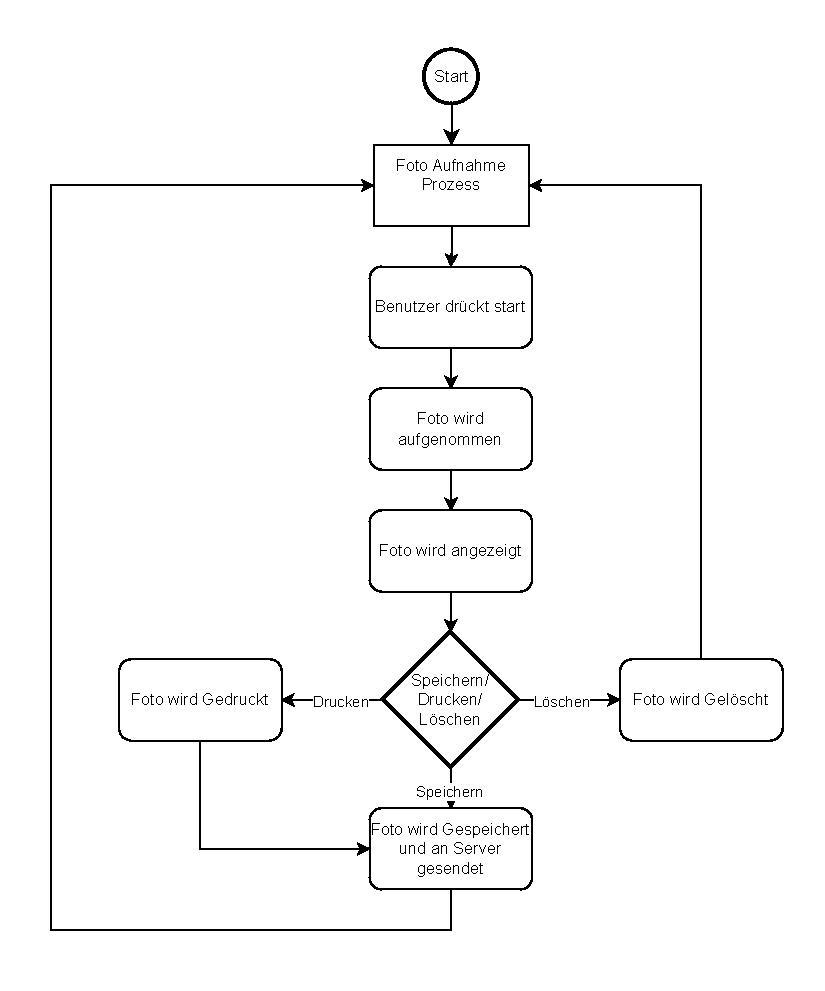
\includegraphics[width=0.75\textwidth]{Ablauf_Foto_Aufnehmen.drawio.pdf}
    \caption{Ablaufdiagramm der Fotoaufnahme.}
    \label{fig:Ablauf_Foto_Aufnehmen}
\end{figure}

In der Abbildung \ref{fig:Ablauf_Foto_Aufnehmen} ist der Ablauf der Fotoaufnahme dargestellt.
Wenn der Benutzer auf den Auslöser drückt, wird ein Foto aufgenommen.
Anschließend wird das Bild auf dem Laptop angezeigt, und der Benutzer hat die Möglichkeit,
auszuwählen, ob das Foto gespeichert, bzw. gedruckt werden soll, oder nicht.

\subsection{Webserver}

\newpage

\subsection{Verwendete Technologien}

In dem folgenden Kapitel werden die Technologien beschrieben, welche ich verwendet habe,
um das Projekt umzusetzen.

\subsubsection{Programmiersprache}
C\# ist eine moderne, objektorientierte Programmiersprache, die von Microsoft entwickelt wurde.
Ich habe, da ich bereits Erfahrung mit C\# habe und diese Sprache sehr viel Flexibilität bietet,
einerseits für die Entwicklung von Desktopanwendungen, als auch für die Entwicklung
von Webservern und sogar Webanwendungen, entschieden.

\subsubsection{ASP.NET Core}
ASP.NET Core ist ein plattformunabhängiges, modulares und leistungsfähiges
Framework zur Entwicklung von Webanwendungen und APIs. Es wurde als Nachfolger
von ASP.NET entwickelt und bietet eine moderne Architektur sowie eine hohe
Performance. Im Projekt dient ASP.NET Core als Grundlage für die Serveranwendung,
welche für die Verwaltung der Benutzer und der aufgenommenen Bilder verantwortlich ist.
Durch die integrierte Unterstützung von Abhängigkeiten, Authentifizierung und RESTful
APIs war ASP.NET Core eine ideale Wahl für die Backend-Entwicklung.

\subsubsection{Blazor}
Blazor ist ein Framework zur Erstellung interaktiver Webanwendungen mit C\#,
das im Rahmen von ASP.NET Core entwickelt wurde. Es ermöglicht die Entwicklung
von Web-UIs mit C\# statt JavaScript. In meinem Projekt habe ich Blazor WebAssembly
verwendet, um eine clientseitige Webanwendung zur Konfiguration und Gestaltung
der aufgenommenen Bilder umzusetzen. Diese Webanwendung läuft direkt im Browser
und kommuniziert über HTTP mit dem Backend.

\subsubsection{Entity Framework Core}
Entity Framework Core ist ein objekt-relationaler Mapper (ORM) für .NET.
Es erlaubt, Datenbankabfragen in C\# zu formulieren, wodurch die Interaktion
mit der Datenbank deutlich vereinfacht wird. In meinem Projekt verwende ich
Entity Framework Core zur Verwaltung und Persistierung von Benutzerdaten sowie
Bildinformationen. Die Verwendung eines ORM trägt außerdem zur Wartbarkeit und
Erweiterbarkeit der Anwendung bei.

\subsubsection{Canon EDSDK}
Zur Ansteuerung der Canon-Spiegelreflexkamera verwende ich das Canon EOS Digital
SDK (EDSDK). Dieses Software Development Kit ermöglicht es, über eine
USB-Verbindung Fotos aufzunehmen und Kameraeinstellungen zu verändern.
Die Integration dieser Schnittstelle in die Anwendung erlaubt es, Bilder direkt
aus der Anwendung heraus aufzunehmen und zu speichern.

\subsubsection{Windows Credential Manager}
Der Windows Credential Manager wird genutzt, um Anmeldedaten wie den Refresh-Token
sicher zu speichern. Dadurch können Benutzer auch nach einem Neustart der Anwendung
automatisch eingeloggt bleiben, ohne ihre Zugangsdaten erneut eingeben zu müssen.

\subsection{Architektonische Konzepte}

In diesem Kapitel werden zentrale Entwurfskonzepte und Prinzipien vorgestellt,
die bei der Umsetzung der Anwendung eine wichtige Rolle gespielt haben.

\subsubsection{Dependency Injection und IoC}
Inversion of Control (IoC) ist ein Prinzip, bei dem die Steuerung über
die Erstellung und Verwaltung von Abhängigkeiten nicht vom Entwickler,
sondern vom Framework übernommen wird. In .NET wird dieses Prinzip durch
Dependency Injection (DI) umgesetzt. Alle Dienste und Komponenten werden im
sogenannten IoC-Container registriert und bei Bedarf automatisch bereitgestellt.
Diese Struktur verbessert die Testbarkeit und Modularität des Codes.

In dem folgenden Code Snippet wird gezeigt, wie eine Abhängigkei, hier die 
Drucker-Klasse in den IoC-Container registriert wird:

\begin{lstlisting}
builder.Services.AddSingleton<IPrinter, Printer>();
\end{lstlisting}    

Wenn die Printer-Klasse nun benötigt wird, kann sie einfach im Konstruktor
einer anderen Klasse injiziert werden:

\begin{lstlisting}
public class ImageManager(IPrinter printer)
{
    private readonly IPrinter _printer = printer;

    public async Task PrintAndSaveAsync(Image<Rgb24> image)
    {
            await SaveAsync(image);

            await printer.PrintAsync(image);
    }
}
\end{lstlisting}

Wenn nun diese ImageManager-Klasse vom IOC Container instanziiert wird,
wird automatisch die Printer-Klasse mit übergeben. Bei diesem Beispiel, 
ist es noch sehr übersichtlich, da nur eine Abhängigkeit vorhanden ist.
Wenn jedoch mehrere Abhängigkeiten vorhanden sind, wird es schnell
unübersichtlich, was durch die Verwendung von Dependency Injection
deutlich vereinfacht wird. Außerdem wird das unnötige Erstellen und
Zerstören von Objekten vermieden, was die Performance der Anwendung
verbessert, da hier die Printer-Klasse nur einmal erstellt wird und
nicht bei jedem Aufruf der PrintAndSaveAsync-Methode neu instanziiert werden muss.

\subsubsection{ILogger und Serilog}

Für das Logging wurde das \texttt{ILogger\textless{}T\textgreater{}}-Interface
aus dem .NET Core Framework verwendet. Dieses Interface ermöglicht eine
einheitliche und flexible Protokollierung, bei der Logeinträge in
unterschiedlichen Formaten und über verschiedene Ausgabemedien
(z.\,B. Konsole, Datei oder Remote-Logging-Dienste) erzeugt werden können 
ganz ohne Anpassungen am Anwendungscode.

Die Bereitstellung des Loggers erfolgt über Dependency Injection.
Jede Klasse kann dadurch eine auf ihren Typ spezialisierte Instanz von
\texttt{ILogger\textless{}T\textgreater{}} erhalten. Das verbessert die
Nachvollziehbarkeit im Log, da jeder Eintrag eindeutig der Herkunftsklasse
zugeordnet werden kann.

Im folgenden Beispiel wird gezeigt, wie Logging in der \texttt{Printer}-Klasse
verwendet wird:

\begin{lstlisting}
public class Printer(ILogger<Printer> logger)
{
    private readonly ILogger<Printer> _logger = logger;

    public Task PrintAsync(Image<Rgb24> image)
    {
        // Drucken des Bildes

        _logger.LogInformation(
            "Bild erfolgreich gedruckt: {imageName}", image.Name);
    }
}
\end{lstlisting}

Zur Ausgabe der Logeinträge wird Serilog als Logging-Provider verwendet.
Die Konfiguration erfolgt bei der Erstellung des Host-Builders:

\begin{lstlisting}
var logger = new LoggerConfiguration()
    .Enrich.FromLogContext()
    .Enrich.WithEnvironmentName()
    .Enrich.WithMachineName()
    .Enrich.WithProperty("Source", "UI")
    .WriteTo.Seq("http://localhost:5341")
    .CreateLogger();

builder.Logging.AddSerilog(logger);
\end{lstlisting}

Die Logs können so flexibel an verschiedene Ziele weitergeleitet werden etwa,
in die Konsole, in lokale Dateien oder an zentrale Logging-Dienste wie Seq.
Dies ermöglicht eine kontinuierliche Überwachung des Systemverhaltens zur
Laufzeit und eine gezielte Analyse im Fehlerfall.

Insgesamt trägt dieses Logging-Konzept entscheidend zur Wartbarkeit und Fehlersuche bei,
da relevante Abläufe und Probleme nachvollziehbar und strukturiert dokumentiert werden.

